\documentclass[12pt, oneside]{article}
\usepackage{geometry}
\usepackage[utf8]{inputenc}
\usepackage{setspace}
\usepackage{times}
\usepackage{url}
\usepackage{multirow}
\usepackage[usegeometry]{typearea}
% Useful for checking layout
% \usepackage{showframe}
\usepackage{fancyhdr}
\usepackage{blindtext}
% Indenting the first sentence after section
\usepackage{indentfirst}
% Set language
\usepackage[german]{babel}
% Abbreviations
\usepackage{glossaries}
% For big tables which span multiple pages
\usepackage{longtable}
% Images
\usepackage{graphicx}
\graphicspath{ {./images/} }
% APA Citation Style
\usepackage[natbibapa]{apacite}
% Smaller font size for captions
\usepackage[font=small,labelfont=bf]{caption}
% Table related packages
\usepackage{booktabs}


\geometry{
 a4paper,
 left=30mm,
 top=25mm,
 right=25mm,
 bottom=20mm,
 footskip=15pt,
}

\setstretch{1.3} % Define Line Spacing
\renewcommand{\headrulewidth}{0pt} % Remove footer line

\pagestyle{fancy} % Allow for customizing header and footer
% Customize footer for page number location
\fancyhf{}
\fancyfoot{}
\fancyhead[R]{Yannick Hutter}
\fancyhead[L]{Exposé}
\fancyfoot[R]{\thepage}



 \makeglossaries

 \newglossaryentry{dsrm}
 {
     name=DSRM,
     description={Design Science Research Model}
 }
 \newglossaryentry{foph}
 {
     name=FOPH,
     description={Federal Office of Public Health}
 }
 \newglossaryentry{fhgr}
 {
     name=FHGR,
     description={Fachhochschule Graubünden}
 }
 \newglossaryentry{svi}
 {
     name=SVI,
     description={Social Vulnerability Index}
 }
 \newglossaryentry{who}
 {
     name=WHO,
     description={World Health Organisation}
 }



\begin{document}
\urlstyle{same}
\pagenumbering{roman}
\begin{titlepage}
	\begin{center}
		\Huge
		\textbf{Exposé}
		
		\vspace{0.5cm}
		\LARGE
		Analyse und Implementierung eines personalisierbaren Corona Dashboard für Millennials
		
		\vspace{1.5cm}
		\normalsize
		\textbf{Yannick Hutter}\\
		\textbf{Digital Business Management Klasse 18tz}\\
		\textbf{Talackerstrasse 8}\\
		\textbf{8887 Mels}\\
		\textbf{yannick.hutter@stud.fhgr.ch}\\

		
		\vfill
		Referrent: Daniel Klinkhammer\\
		Korefferent: Michael Burch\\
		
		\vspace{0.8cm}
		
		
		Digital Business Management\\
		Fachhochschule Graubünden\\
		Mels, Mai 2022
	\end{center}
\end{titlepage}



\tableofcontents
\listoffigures
\listoftables

\clearpage
\printglossaries



\clearpage
\pagenumbering{arabic}
\setcounter{page}{3}

\section{Einleitung}
Die Coronavirus-Pandemie (fortlaufend als Corona bezeichnet) hat in grossen Teilen der Welt seine Spuren hinterlassen. So geht gemäss dem \Gls{foph} hervor, dass im Zeitraum vom 24.02.2020 bis zum 10.03.2022 mehr als 3 Millionen Ansteckungen in der Schweiz, sowie im Liechtenstein verzeichnet worden sind ~\citep{FOPH.13.03.2022}. Ein wichtiges Mittel zur Kommunikation mit der Bevölkerung sind hierbei Datenvisualisierungen, insbesondere Dashboards.\\

Gemäss Ivankovic ist ein Dashboard eine Ansammlung von Datenvisualisierungen, womit der Nutzer die für ihn relevantesten Informationen auf einen Blick erkannt und entsprechend darauf reagieren kann. Im Gegensatz zu klassischen Medien wie Reports erlauben Dashboards die Darstellung von Daten in Echtzeit. Dies ist besonders in einer weltweiten Pandemie von grosser Bedeutung, da somit relevanten Stellen schneller informiert und Zielgruppen entsprechend sensibilisiert werden können ~\citep[S. 2]{Ivankovic.2021}. Die Wichtigkeit von Dashboards, besonders zu Beginn der Pandemie, bestätigt ebenfalls die Studie von Barbazza. Diese zeigt auf, dass während der Anfangszeit der Pandemie (Februar - Mai 2020) die grösste Anzahl von Corona Dashboards erstellt worden ist ~\citep[S. 8]{Barbazza.2021}.\\

Ein Dashboard, welches versucht ein globales Bild wiederzugeben, ist das WHO Coronavirus Dashboard ~\citep{WHO.23.04.2022}. Auf diesem Dashboard sind Ansteckungszahlen, Todesfälle sowie Impfquoten von mehreren Ländern ersichtlich. Dass die Erstellung von Corona Dashboards selbst internationale Organisationen wie die \Gls{who} involvierte, soll aufzeigen, wie wichtig Visualisierungen und insbesondere Dashboards während einer weltweiten Pandemie geworden sind.
\clearpage

\section{Forschungsfrage}
Die Landschaft der Corona Datenvisualisierungen ist sehr breit gestrickt und umfasst unterschiedlichste Repräsentanten von Visualisierungsarten. Nebst den einzelnen Visualisierungen wie Liniendiagramme, welche den zeitlichen Verlauf von einzelnen Variablen (zum Beispiel Corona Ansteckungszahlen) aufzeigen, werden diese aber auch in Form von Dashboards zusammengefasst. Eine grosse Anzahl dieser Dashboards sind jedoch  allgemein gehalten und fokussieren sich auf die breite Öffentlichkeit oder Datenanalysten ~\citep[S. 14]{Barbazza.2021}. Auch gibt es von der Nutzerseite her \textit{wenig Personalisierungsmöglichkeiten}. Anpassungen an bereits erstellten Dashboards (zum Beispiel dynamisches Hinzufügen und Enfernen von Visualisierungen) durch die Zielgruppe sind in der Regel nicht vorgesehen. Interessant in diesem Kontext ist es zu untersuchen, wie sich eine spezifische Nutzergruppe ein \textbf{personalisierbares} Corona Dashboard vorstellt und welche \textbf{Informationen} beziehungsweise \textbf{Visualisierungsarten} von Relevanz sind. Aufgrund dieser explorativen Fragestellung ergibt sich folgende übergeordnete Forschungsfrage:


\begin{center}
\textbf{Wie stellen sich Millennials ein personalisierbares Corona Dashboard vor?}
\end{center}

Um diese Forschungsfrage abzudecken, wurden folgende untergeordnete Fragestellungen formuliert:

\begin{center}
\textbf{Welche Visualisierungstypen in Bezug auf Corona werden von Millennials gefordert?\\
(untergeordnete Forschungsfrage 1)}
\end{center}

\begin{center}
\textbf{Welche Informationen in Bezug auf Corona werden von Millennials gefordert?\\
(untergeordnete Forschungsfrage 2)}
\end{center}

\begin{center}
\textbf{Welche Personalisierungsmöglichkeiten in Bezug auf Dashboards werden von Millennials gefordert?\\
(untergeordnete Forschungsfrage 3)}
\end{center}

\clearpage
\section{Methodische Vorgehensweise}
\subsection{Methodik}
Da es sich bei der übergeordneten Forschungsfrage um eine Fragestellung mit explorativem Charakter handelt, wird für die Methodik das \Gls{dsrm} Prozess Model nach Peffers verwendet (siehe Abbildung 1).


\begin{figure}[ht]
	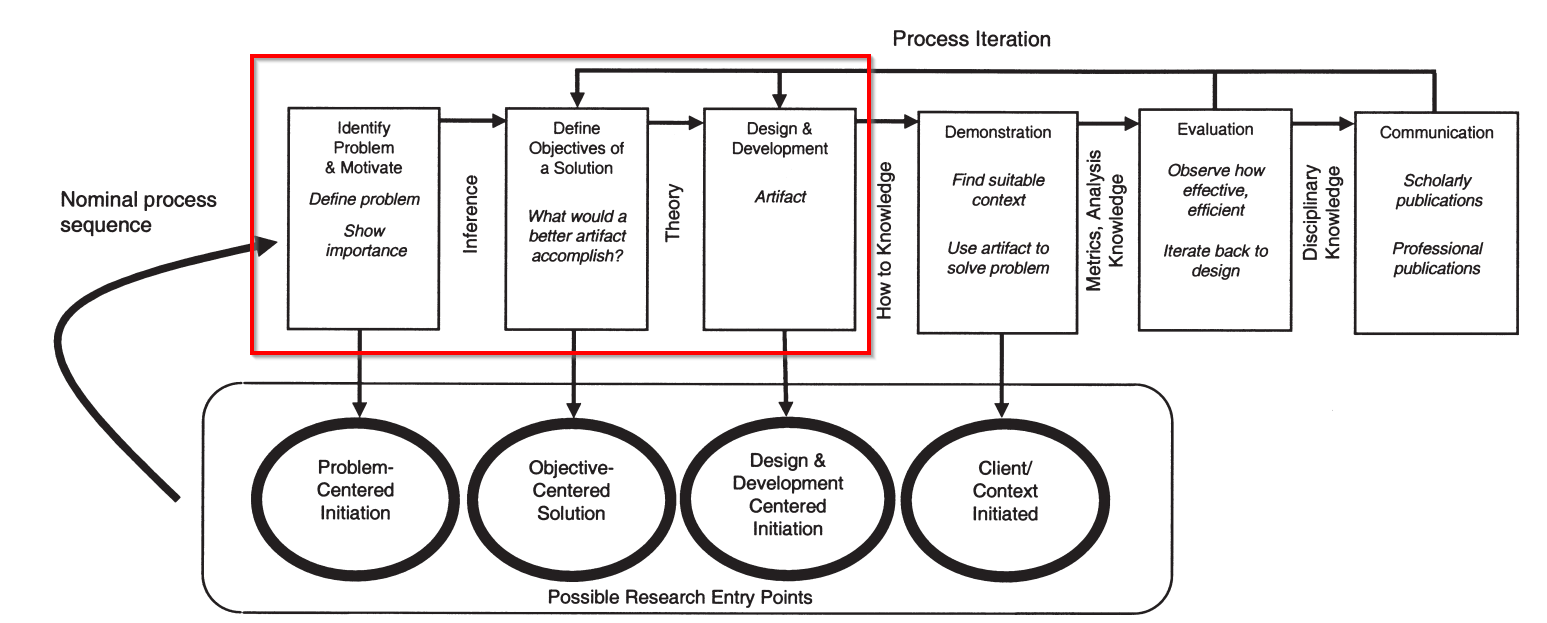
\includegraphics[width=12cm]{images/peffers_dsr_model.png}
	\centering
	\caption{DSRM Prozess Modell nach Peffers ~\citep{K.Peffers.2007}}
\end{figure}

Bei diesem Modell gibt es mehrere Einstiegsmöglichkeiten (siehe \textit{Possible Research Entry Points}). Der Einstiegspunkt für die vorliegende Arbeit bildet der Punkt \textbf{Problem-Centered Initiation}. Als erstes wird der Schritt \textit{Identify Problem and Motivation} angegangen. Das Ziel hierbei ist es, dass eigentliche Problem zu identifizieren und die eigene Motivation für eine Lösung zu begründen. Das Problem, welches gelöst werden soll, ist die die starre Natur bestehender Corona Dashboards in Bezug auf Personalisierungsmöglichkeiten. In diesem Kontext ist die Entwicklung eines Prototyps interessant, welcher die Erstellung der Dashboards \textbf{in die Hände der Zielgruppe selbst legt} und so auch individuelle Personalisierungs- und Anpassungsmöglichkeiten bietet.

Im zweiten Schritt \textit{Define Objective of a Solution} geht es darum, das Ziel einer möglichen Lösung aufzuzeigen. Anschliessend geht es im Schritt \textit{Design und Development} um die eigentliche Erstellung des Artefakts, was im Zuge dieser Arbeit ein High Fidelity Prototyp darstellt. In den nächsten Schritten wird die Evaluation des erstellten Prototyps, sowie die Publikation der Ergebnisse behandelt. Jedoch beschränkt sich die vorliegende Arbeit auf die Erstellung eines Prototyps aufgrund teilstrukturierter Interviews mit Millennials. Die eigentliche Evaluation des Prototyps kann im Rahmen einer weiterführenden Arbeit evaluiert werden.

\clearpage
\subsection{Vorgehen}
Eine Visualisierung stellt eine gewisse \textit{Information} in einer leicht verständlichen und anschaulichen Weise dar. In einem ersten Schritt muss also die notwendige Information, welche die Grundlage für die Visualisierung darstellt, evaluiert werden. Hierzu wird das Codebook von Zhang verwendet ~\citep{YixuanZhang.2021}. Zhang untersuchte in seiner Studie \textit{Mapping the Landscape of COVID-19 Crisis Visualizations} eine Vielzahl von unterschiedlichen Corona Datenvisualisierungen und teilte diese in verschiedene Nachrichtenkategorien ein (siehe Abbildung 2).

\begin{figure}[ht]
	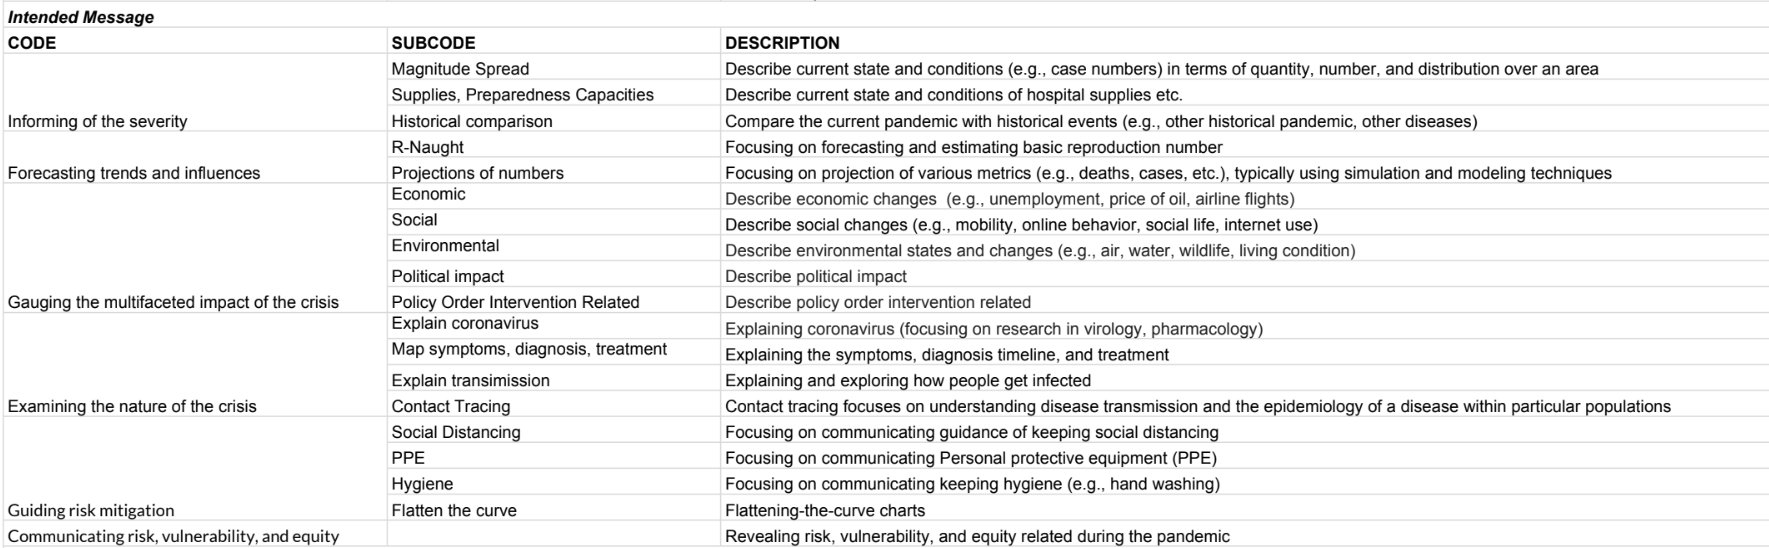
\includegraphics[width=14cm]{images/message_categories_zhang.png}
	\centering
	\caption{Ausschnitt zur Erklärung des Codebooks von Zhang ~\citep{YixuanZhang.2021}}
\end{figure}

Das Codebook beinhaltet zudem Informationen über die Visualisierungsarten (Balkendiagramm etc.), sowie entsprechende Internetquellen. Aus dem Codebook kann daher ermittelt werden, welche Datenvisualisierungen für welche Information (Nachrichtenkategorie) verwendet worden sind. Hierfür wurde im Vorfeld bereits eine Auswertung des Codebooks mittels eines erstellten Jupyter Notebooks gemacht\footnote{\url{https://github.com/YahArt/covid-jupyter-notebook-fhgr}}.

\clearpage
Somit ist bekannt, welche Visualisierungsarten wie häufig für welche Nachrichtenkategorie inkl. Subkategorien verwendet worden sind (siehe Abbildung 3).


\begin{figure}[ht]
	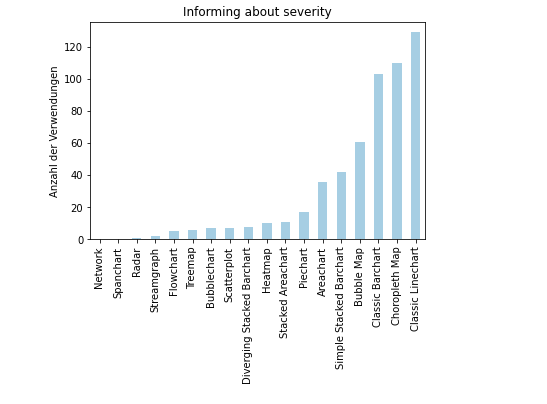
\includegraphics[width=9cm]{images/visualization_types_for_magnitude_spread.png}
	\centering
	\caption{Beispiel einer Auswertung mit Hilfe des erstellten Juypter Notebooks, welche die Visualisierungstypen für die Nachrichtenkategorie \textit{Informing of the severity} aufzeigt (Eigene Darstellung)}
\end{figure}

Für das eigentliche Vorgehen werden \textit{teilstrukturierte Interviews} durchgeführt. Hierzu werden die Probanden zuerst danach befragt, über welche Informationen (Nachrichtenkategorie) Sie sich informieren würden. Anschliessend wird mit den Subkategorien (Subcode) die genaue Art der Information festgehalten. Zusätzlich müssen die Probanden die für sie passende Datenvisualisierung auswählen. Die Auswahl der Visualisierung pro Subkateogrie etc. ist aufgrund der Voranalyse durch das erstellte Jupyter Notebook möglich. Somit können die ersten zwei untergeordneten Forschungsfragen beantwortet werden. Um die dritte untergeordnete Forschungsfrage zu beantworten, werden die Probanden darum gebeten auf ein bestehendes Corona Dashboard zu navigieren. Anschliessend werden verschiedene Fragen in Bezug auf die Struktur, das Aussehen sowie Anpassungsmöglichkeiten gestellt. Dieser Teil des Interviews ist sehr explorativ und soll daher mit Hilfe des \textit{think-aloud Ansatz} erfolgen. 

Das durchgeführte Interview bildet im Anschluss die Grundlage für die Erstellung eines \textit{High-Fidelity Prototyps}.


\clearpage
\subsection{Aufbau}
Die Arbeit orientiert sich wie bereits erwähnt an den ersten drei Phasen des DSR Modells von Peffers. Dieses Vorgehensmodell soll sich auch in der Struktur der Arbeit wiederfinden.\\

\textbf{Einleitung}
\begin{itemize}
    \item Kontextabgrenzung
    \item Stand der Forschung
    \item Forschungsfrage
    \item Methodisches Vorgehen\\
\end{itemize}

\textbf{Corona Dashboards (Theoriekapitel)}
\begin{itemize}
    \item Begriffsdefinition
    \item Arten von Dashboards
    \item Aufbau und Funktionsweise von Dashboards\\
\end{itemize}


\textbf{Problemidentifizierung und Motivation (Identify Problem und Motivation)}
\begin{itemize}
    \item Problemidentifikation
    \item Motivation – Erstellung eines personalisierbaren Corona Dashboard für Millennials\\
\end{itemize}

\textbf{Identifikation der Ziele (Define Objectives of a Solution)}
\begin{itemize}
    \item Erstellung des Untersuchungsinstrumentes
    \item Identifikation von relevanten Informationen
    \item Evaluation von Visualisierungstypen für Corona Dashboards
    \item Identifikation von relevanten Personalisierungsmöglichkeiten in Bezug auf Dashboards\\
\end{itemize}

\textbf{Design und Development}
\begin{itemize}
    \item Design mittels Sketching
    \item High-Fidelity Prototyp als Web Applikation\\
\end{itemize}

\textbf{Reflexion und Limitationen}

\clearpage
\section{Stand der Forschung}
Die Coronavirus-Pandemie greift seit ihrem Aufkommen in eine Vielzahl von Lebensbereichen ein. Es ist wenig verwunderlich, dass zu einem solch einschneidendem Thema eine grosse Anzahl von wissenschaftlichen Publikationen erstellt worden sind. Die bereits angesprochene Studie von Zhang (siehe Kapitel 3.2) zeigt hierbei die breit strukturierte Landschaft der Corona Datenvisualisierungen auf und weisst den Visualisierungen verschiedene Nachrichtenkategorien zu ~\citep{YixuanZhang.}. Die Studie von Ivankovic setzt sich mit \textit{webbasierten Corona Dashboards} auseinander und leitet Design Guidelines für ab ~\citep{Ivankovic.2021}. Auch wurde bereits im Zuge einer Studie die Schwierigkeiten bei der Erstellung von Corona Dashboards aus dem Blickwinkel der eigentlichen Ersteller evaluiert ~\citep{Barbazza.2021}. Jedoch scheint es zum jetzigen Zeitpunkt noch keine Studie zu geben, welche die Erstellung von personalisierbaren Corona Dashboards für eine bestimmte Zielgruppe, unter Berücksichtigung eines nutzerzentrierten Vorgehens, untersucht.

\clearpage
\bibliographystyle{apacite}
\bibliography{main.bib}

\clearpage
\section*{Anhang}
\begin{table}[ht]
\begin{tabular}{@{}p{4cm}p{4cm}p{6.5cm}@{}}
\toprule
\textbf{Quelle}                                          & \textbf{Schlüsselwörter}        & \textbf{Artikel} \\ \midrule
\url{https:\\scholar.google.com}                         & covid dashboard                 & ~\citep{Dong.2020}         \\ \midrule
                                                         &                                 & ~\citep{Florez.2020}       \\ \midrule
                                                         &                                 & ~\citep{Berry.2020}        \\ \midrule
                                                         & user centered dashboards        & ~\citep{Francois.2021}     \\ \midrule
                                                         &                                 & ~\citep{Young.2020}        \\ \midrule
                                                         & customizable dasbhoards         & ~\citep{Roberts.2017}      \\ \midrule
\url{https:\\dl-acm.org}                                 & covid19 dashboard               & ~\citep{Vitale.}           \\ \midrule
                                                         & evaluating crisis dashboards    & ~\citep{Ivanov.2018}       \\ \midrule
                                                         & data dashboards                 & ~\citep{Maheshwari.}       \\ \midrule
                                                         &                                 & ~\citep{Beheshti.}         \\ \midrule
\url{https:\\google.com}                                 & covid dashboard evaluation      & ~\citep{Barbazza.2021}         \\ \midrule
                                                         & how user use covid19 dashboards & ~\citep{Ivankovic.2021}    \\ \bottomrule
\end{tabular}
\caption{\label{tab:research-protocol}Rechercheprotokoll (Eigene Darstellung)}
\end{table}
\clearpage


\subsection*{Zeitplan}

\begin{table}[ht]
\begin{tabular}{@{}p{13cm}p{2cm}@{}}
\toprule
\textbf{Tätigkeit}                                                                                & \textbf{Stichtag} \\ \midrule
Erstellung des Untersuchungsinstrumentes                                                          & 08.05.2022        \\ \midrule
Kapitel Einleitung fertig stellen                                                                 & 08.05.2022        \\ \midrule
Theoriekapitel fertig stellen & 15.05.2022        \\ \midrule
Kapitel Problemidentifizierung und Motivation fertig stellen                                      & 15.05.2022        \\ \midrule
Durchführung der teilstrukturierten Interviews mit Hilfe des erstellten Untersuchungsinstrumentes & 29.05.2022        \\ \midrule
Abgabe Exposé                                                                                     & 22.05.2022        \\ \midrule
Kapitel Identifikation der Ziele fertig stellen                                                   & 05.06.2022        \\ \midrule
Implementierung Prototyp                                                                          & 26.06.2022        \\ \midrule
Kapitel Design und Development fertig stellen                                                     & 26.06.2022        \\ \midrule
Kapitel Fazit fertig stellen                                                                      & 03.07.2022        \\ \midrule
Kapitel Reflexion und Limitation fertig stellen                                                   & 10.07.2022        \\ \midrule
Korrekturlesung und Verbesserung                                                                  & 24.07.2022        \\ \midrule
Abgabe Thesis                                                                                     & 25.07.2022        \\ \bottomrule
\end{tabular}
\caption{\label{tab:time-table}Zeitplan (Eigene Darstellung)}
\end{table}


\clearpage
\section*{Eigenständigkeitserklärung}
Hiermit bestätigt der Verfasser, dass die vorliegende Arbeit selbstständig verfasst und keine anderen als die angegebenen Hilfsmittel benutzt wurden. Stellen der Arbeit, die dem Wortlaut oder dem Sinn nach anderen Werken entnommen sind, wurden unter Angaben der Quelle kenntlich gemacht.

\begin{figure}[ht]
	
\includegraphics[width=6cm]{images/signature.png}
\end{figure}
Yannick Hutter, Mels am 17. Mai 2022

\end{document}